% Activate the following line by filling in the right side. If for example the name of the root file is Main.tex, write
% "...root = Main.tex" if the chapter file is in the same directory, and "...root = ../Main.tex" if the chapter is in a subdirectory.
 
%!TEX root =  testMain.tex

\chapter[Simple Spatial Simulations]{A Simple Robbery - Spatial Simulations and their Bayesian Networks}

 The problem is that in the previous chapter, we have established that we have a method to convert a simple forward-chaining simulation into a collection of data, which then in turn can be used to create a Bayesian Network, that represents the situation in the simulation.
 
 However, this was totally 100\% determined by deterministic forward chaining rules. The real world does not run on deterministic forward chaining rules (as far as we know). At least, we are spatially situated, which means that there are probabilities that will arise out of interactions between agents and their environment. These probabilities are not `set' in the same ways as the probabilities are set in the previous chapter, they arise organically from interactions: an agent has to be located at a door to break in, an agent can be seen by a camera only in some locations of the simulation. We do not know these probabilities a-priori.
 
 Research questions for this chapter:
 
 \begin{itemize}
 \item Can we create an automatic BN from a simulation of similar accuracy and rmse as in the previous chapter, but now spatially explicit, with agents, and with evidence?
 \item What is the effect of loss of precision on this network?
 \item What is the effect of truly private knowledge on the network?
 \end{itemize}
 


\section{Experiment 1: Generating BNs and lowering precision}

For the first experiment, a very simple crime case will be modelled in a multi-agent simulation. This is the data-generating environment, the gathered data will be used by the K2 algorithm to automatically generate a Bayesian Network. This network will be assessed based on the criteria set out in chapter 3.  

\subsection{Introduction}

The scenario that the agents play out goes as follows. There are two agents. They are neighbors. One day, the agent who lives in the house on the right ($R$), walks past the house of the other agent ($L$). $R$ looks inside, if it can. Sometimes it cannot look inside, because $L$ has drawn the curtains. However, if $R$ can look inside, it might see a goodie in the house. It also might not see a goodie, if $L$ has lost the goodie - in that case, the goodie has been lost. However, if the goodie is there, $R$ will know that the goodie is there. Then, because $R$ is a rational agent, it will try to calculate the worth of the object, and if it might want to steal it. It can decide to target the object. If $R$ knows and targets the object, $R$ has a motive. Then, $R$ attempts to break into the house by breaking the lock on the door, grabbing the goodie, and running away to its own house.  Meanwhile, $L$ is returning home. If $R$ thinks that $L$ might have seen it stealing, $R$ will flee home, with or without the goodie. $L$ has also hung up security cameras on the outside corner of its house, that might serve as evidence against $R$.

With regards to the end, there can be three outcomes: either the goodie is lost, the goodie is not lost but was stolen successfully, or the goodie is not lost and wasn't stolen successfully. %({\color{red}does this mean that there was always a stealing attempt? check in jup}). 
The environment of the agents is very simple, just two `houses' (rectangles, really). The environment and the agents (with their vision parameter) are shown in Figure~\ref{env}.

\begin{figure}[htbp]
\begin{subfigure}{.5\textwidth}
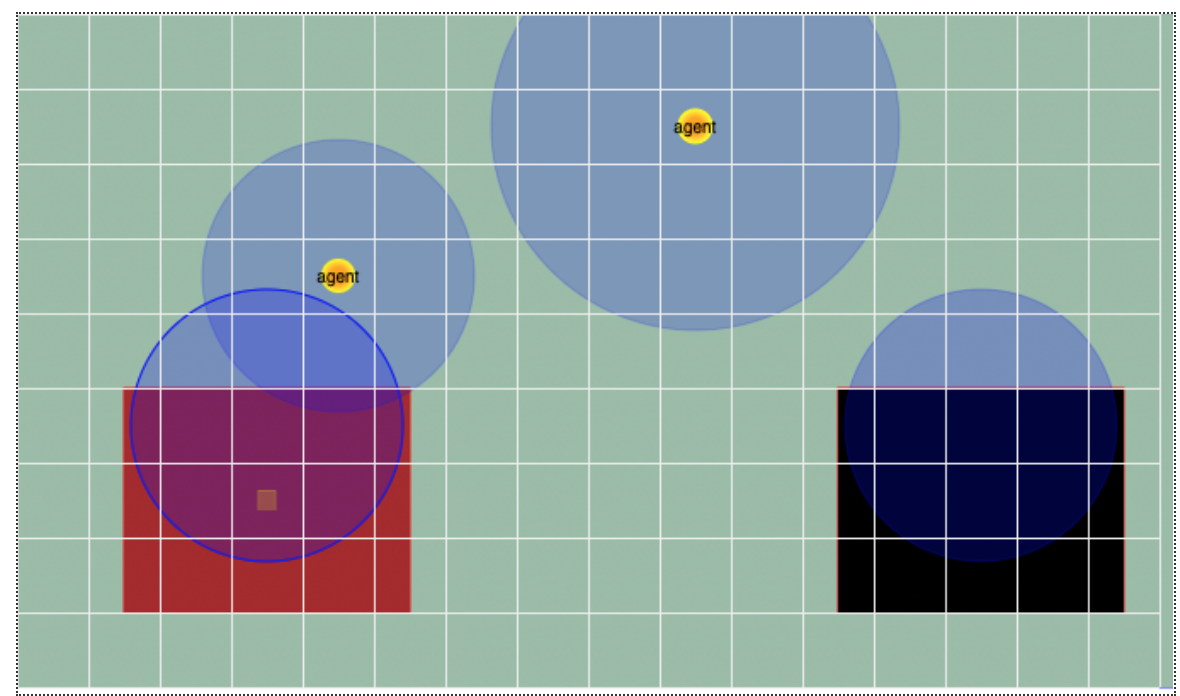
\includegraphics[width=\linewidth]{images/sim1.png}
\caption{The simulation with the 2 agents.}
\end{subfigure}
\begin{subfigure}{.5\textwidth}
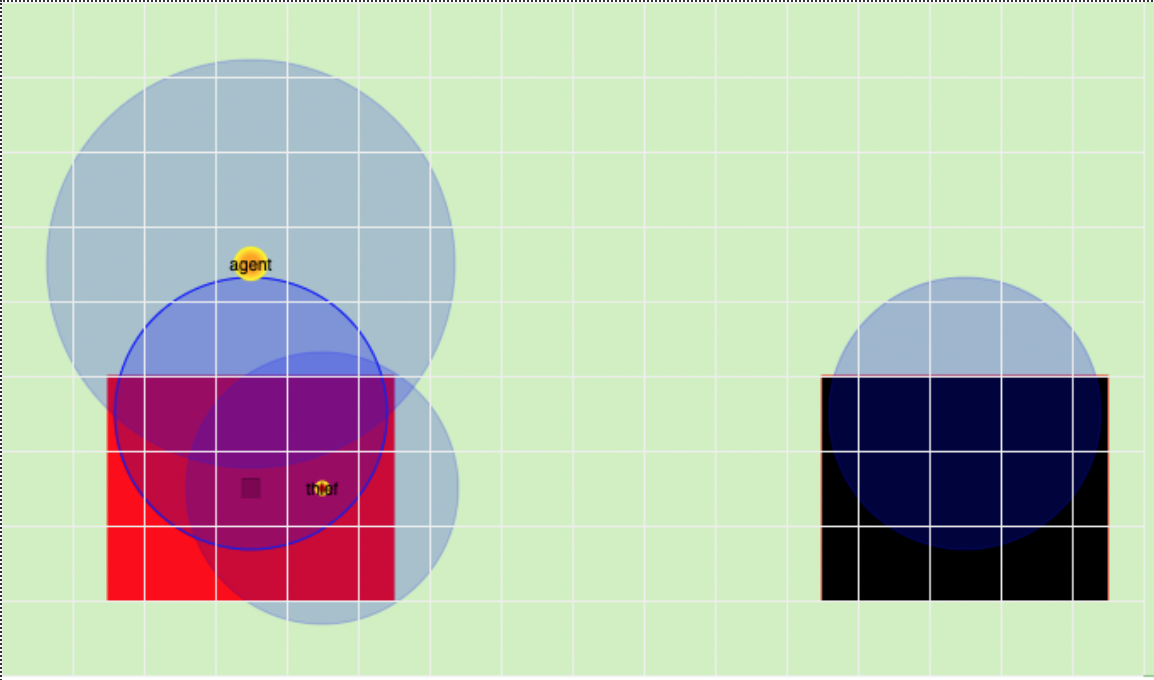
\includegraphics[width=\linewidth]{images/stealing.png}
\caption{The agent attempts to steal something but flees when it thinks that it is noticed.}
\end{subfigure}
\caption{Agents behaving badly in simulation.}
\label{env}
\end{figure}

\subsection{Methods}
There are four things to be explained here: the agent behaviour, the operationalisation of the random variables, the simulation (meta-)parameters, and the process through which the cpts of the given BN is to be disturbed. The simulation was ran for 2000 times, with 30 epochs max per run.

\subsubsection{Agent behaviour}
flowchart here.

\subsubsection{Operationalisation of the RVs}

The operationalisation of the random variables is very important. In the table below are all the reporters and how they are defined.

\begin{adjustbox}{center}
\footnotesize
\centering
\begin{tabular}{|l|l|}
 \hline
 RV &Operationalization\\
 \hline
lost\_object   & A random number generator (0, 1) generates a number. If the number $\leq 0.2$, the object is lost.\\
curtains & A random number generator (0, 1) generates a number. If the number $\leq 0.8$, the house has no curtains.  \\
raining & A random number generator (0, 1) generates a number. If the number $\leq 0.5$, it is raining.   \\
know\_object & if we see an object in our vision that is not our own, and we are not already targeting some`
thing else  \\
target\_object & if we know the object exists, and we consider the value of the object higher than our risk threshold.  \\
motive & if we have a target \\
compromise\_house & if we are adjacent to the target's house's door, and we have a breaking and entering skill of greater than 5. \\
flees\_startled & if we see another agent and we haven't been observed yet  \\
successful\_stolen & if we're not in someone's house anymore and we have the object in our possession \\ 
E\_s\_spotted\_by\_house&  {\color{red} todo fill in}. \\ 
E\_disturbed\_house&   \\ 
E\_object\_is\_gone&   \\ 
E\_broken\_lock&   \\ 
E\_s\_spotted\_with\_goodie&   \\ 
E\_private&   \\ 
\hline
\end{tabular}
\end{adjustbox}


\subsection{Results}

See Figure~\ref{laptop}

\begin{figure}[htbp]
\begin{center}
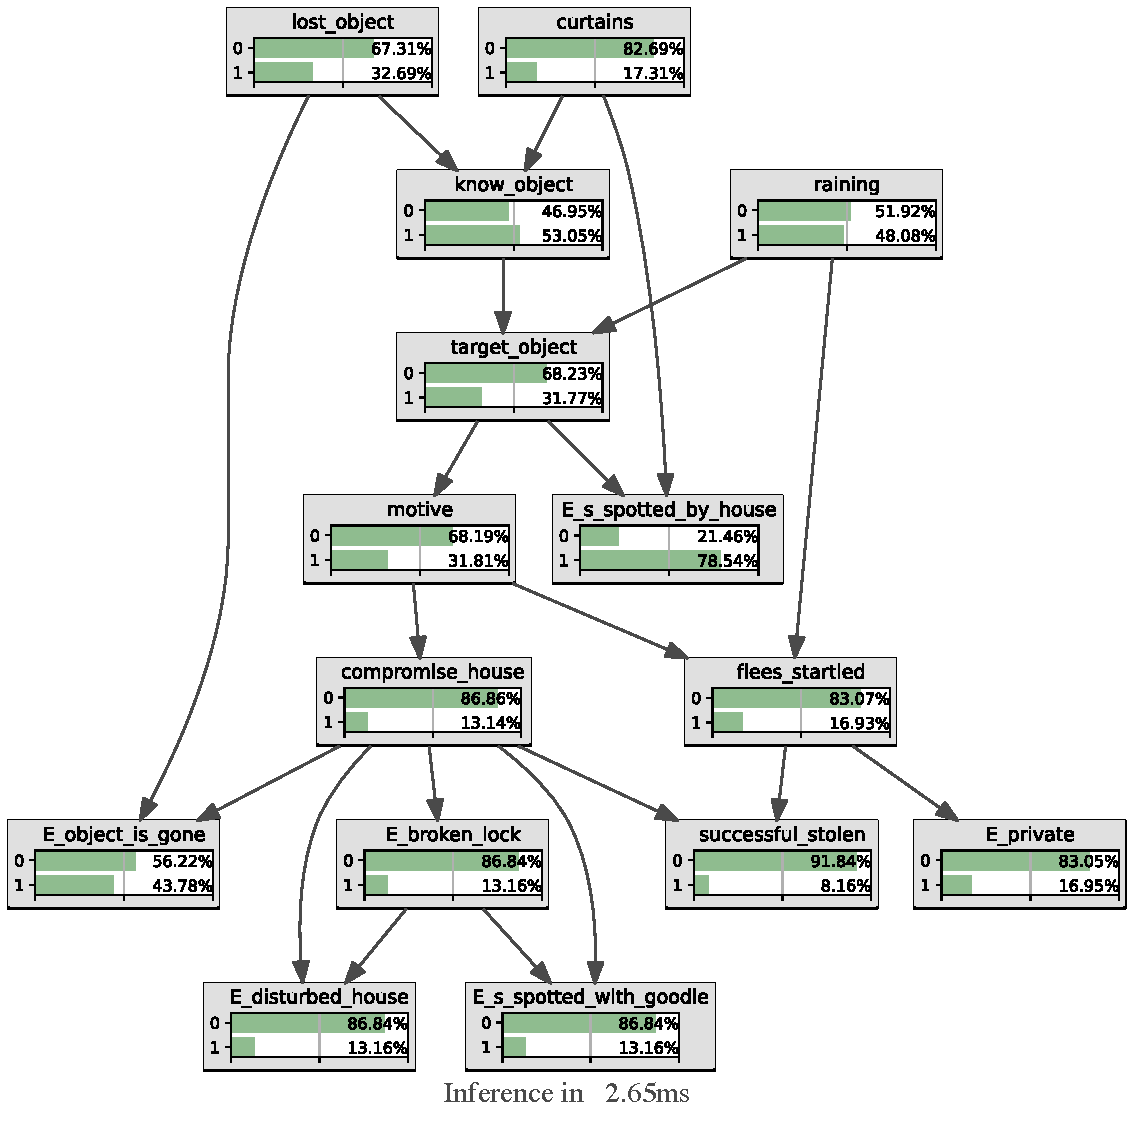
\includegraphics[width=\linewidth]{../experiments/StolenLaptop/bnImage/BNIMAGEStolenLaptop.pdf}
\end{center}
\caption{network structure}
\label{laptop}
\end{figure}


\subsection{Evaluation with regards to structural, performance and human-factor criteria}
In this section, the evaluation criteria as set out before are applied to the networks.

\subsubsection{Structural Criteria}
\begin{enumerate}
\item \textbf{Hypotheses are ordered temporally.}

The main scenario hypothesis nodes are ordered temporally.

\item \textbf{Evidence connects to hypotheses.}

All evidence is connected to at least one hypothesis. However, the structure of how the evidence nodes are added is confusing and overwhelming. One piece of evidence - the most crucial one, which is that the evidence is gone, has 5 parents!

\item \textbf{Relevance: All relevant events are in the BN, all irrelevant events are outside of the BN.}

We know that truly irrelevant nodes are kept out of the main Bayesian Network - we can see that the node for `raining' is not connected to any other node. This is because the rain does not affect anything in this simulation - this is reflected in the Bayesian Network.

\item \textbf{Independent events are not connected to each other.}

Evidence is connected to each other. This is because we need to consider dependent evidence as dependent in the network (I know i read this somewhere, there was a good example with cameras, Fenton?? I forgot!! fucl). 

\end{enumerate}


%%%%%%% Criteria %%%%%%%%
\subsubsection{Performance Criteria}
We consider the accuracy and root mean square per network, then also look at the correspondence, sensitivity values and the progression given a certain evidence set.
\begin{enumerate}
\item \textbf{Accuracy and Root Mean Square error}

The accuracy of the network is 88\% and Root Mean Square error is 0.14. This is comparable to the networks in the previous chapter.

\item \textbf{Correspondence.}

Once again, compared the probabilities in the network with the frequencies of the events in the simulation (maybe run again, larger training set but don't actually train on it). We see the same pattern (Table~\ref{test}) as before, it is accurate within ±0.005. 

\begin{table}
\centering
\begin{tabular}{|c|c|c|}
 \hline
 Conclusion & Frequency P(event) & P(event)\\
 \hline
lost\_object   & 0.1985 & 0.1987\\
curtains & 0.1695 &  0.1697\\
raining & 0.5085 &  0.5085\\
know\_object & 0.6515 &  0.6510\\
target\_object & 0.3135 & 0.3134\\
motive & 0.3135 & 0.3133\\
compromise\_house & 0.0925 & 0.0925 \\
flees\_startled & 0.1655 &  0.1654\\
successful\_stolen & 0.05 & 0.0438\\ 
E\_s\_spotted\_by\_house&  0.901 & 0.9004 \\ 
E\_disturbed\_house& 0.071 &  0.0709\\ 
E\_object\_is\_gone&  0.281 &  0.2793\\ 
E\_broken\_lock&  0.0925 &  0.0924\\ 
E\_s\_spotted\_with\_goodie& 0.083  & 0.0813 \\ 
E\_private&  0.1655 & 0.1653\\ 
\hline
\label{test}
\end{tabular}
\caption{Correspondences}
\end{table}


\item \textbf{Sensitivity analysis values}

\item \textbf{Effect of evidence on the posterior.}

The effect of turning on evidence on the posterior of the initial network is shown in Figure~\ref{baseposterior}.

The scenario that this posterior progression corresponds to is as follows: the duped agent comes home, and finds that their object is gone. Then, it takes a closer look at the door, and sees that the lock is broken. It looks at the disturbed house, and then at the cameras. The camera shows that the other agent was spotted near the house, and later on emerged with the object. Then, we need to look inside the head of the stealing agent, who fled before they saw the duped agent come home - hence, E\_private is 0.

\begin{figure}[htbp]
 \centering
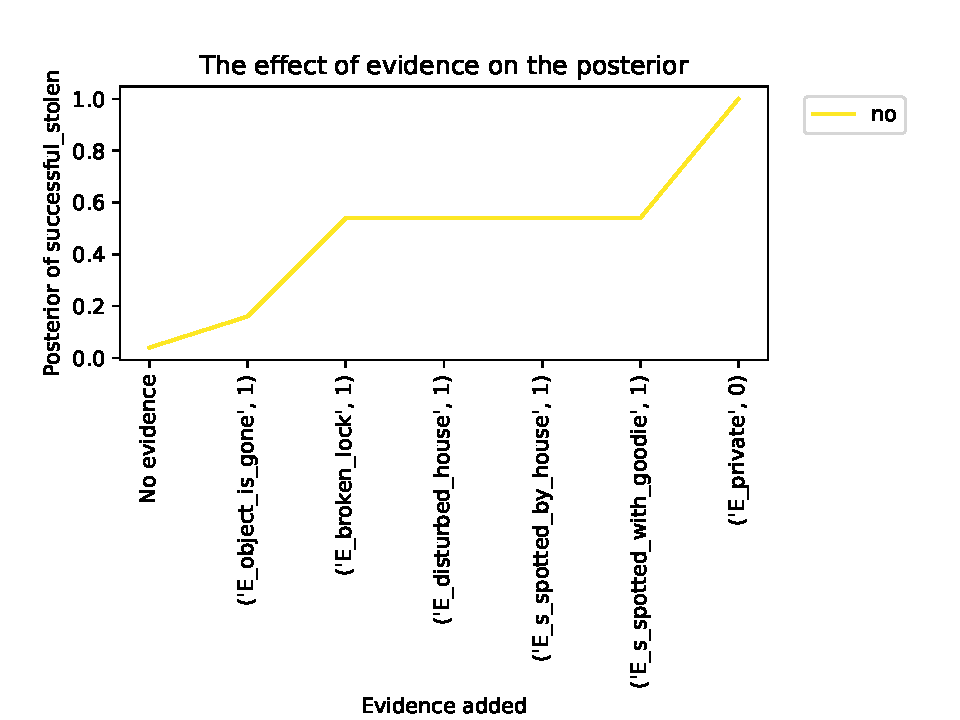
\includegraphics[width=0.6\linewidth]{../experiments/StolenLaptop/plots/posterior_base_networkStolenLaptop.pdf}
\caption{ Progression of evidence resulting in changing the posterior}
\label{baseposterior}
\end{figure}%


\end{enumerate}

\subsubsection{Human Criteria}
\begin{enumerate}
	\item \textbf{How robust is the network against a loss of precision?}

	We again create networks with lower precision, and use the $\epsilon$ method to create networks that do not saturate with 1 or 0, like in the previous chapter. Then we calculate accuracy and root mean square errors on lower-precision networks (Figure~\ref{dist}). We again see that while the RMSE increases when we lose precision, it does not increase by much - from 0.14 to 0.20. This means that the rounding to $\epsilon$ and $1-\epsilon$ instead of 0 or , leaves the network very robust - the accuracy remains the same. So this method works even for more complex networks that include evidence. 

	The posterior progression is also relatively the same as the original network (Figure~\ref{post}).
	\item \textbf{Could a human find these probabilities?}
	\item \textbf{ Can a human determine the correct independence relations?}
\end{enumerate}

\begin{figure}[htbp]
\begin{center}
\begin{subfigure}{.5\textwidth}
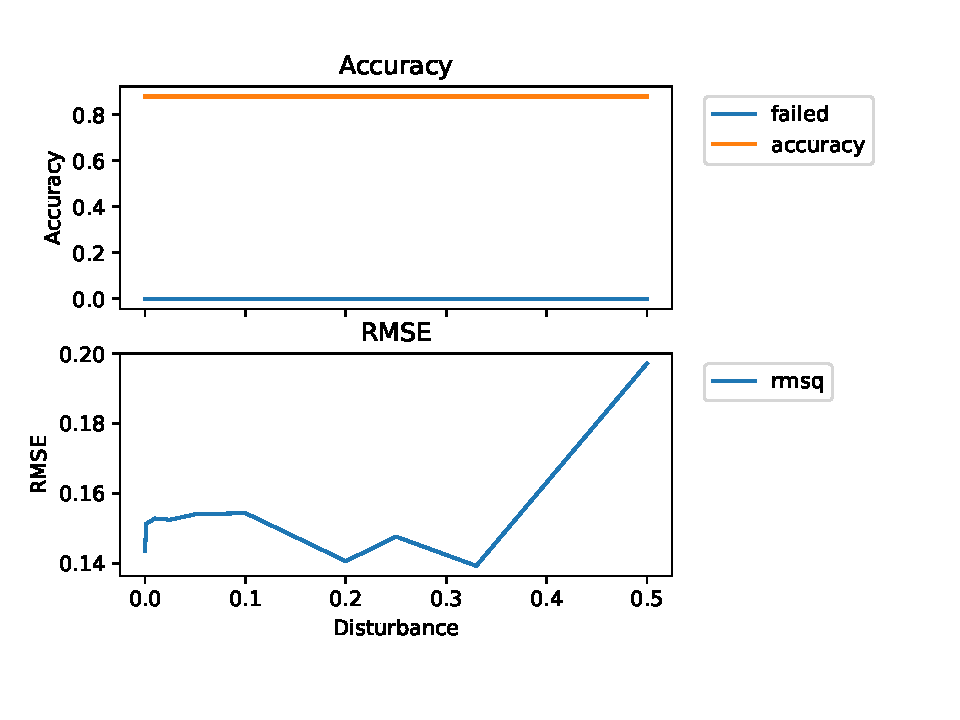
\includegraphics[width=0.9\linewidth]{../experiments/StolenLaptop/plots/performance_StolenLaptop.pdf}
\caption{Network Under Disturbance.}
\label{dist}
\end{subfigure}%
\begin{subfigure}{.5\textwidth}
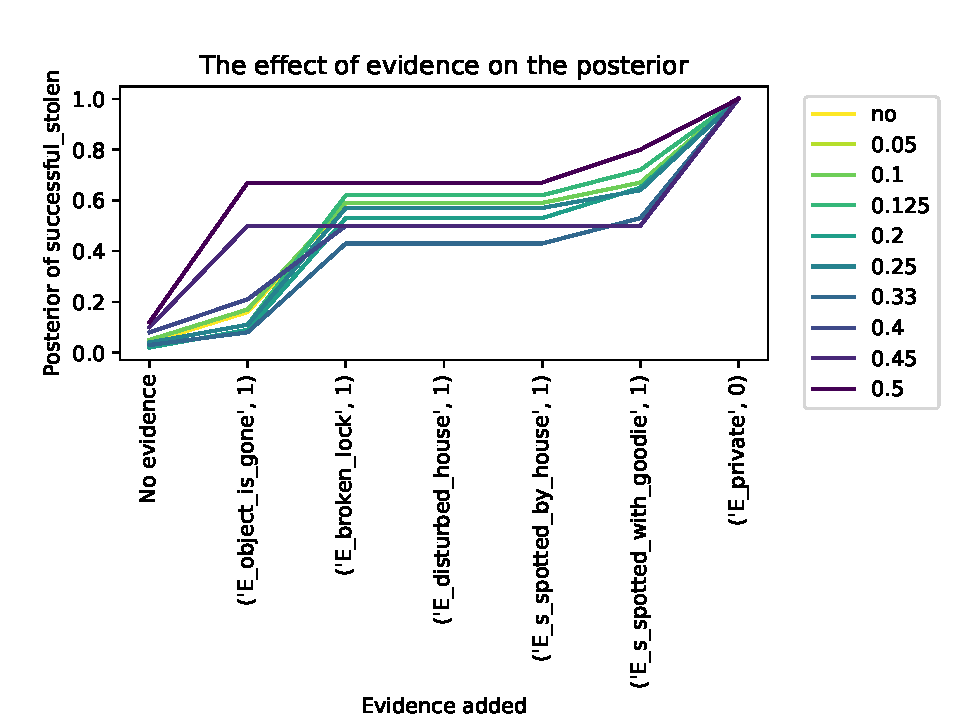
\includegraphics[width=0.9\linewidth]{../experiments/StolenLaptop/plots/posterior_StolenLaptop.pdf}
\caption{ Progression of evidence resulting in changing the posterior}
\label{post}
\end{subfigure}
\end{center}
\end{figure}



\subsection{Discussion}

The network itself makes sense. The spurious node `raining' is not connected to any other node, because the rain should not affect what happens.

The fact that these networks can be rounded without losing accuracy, means that even with a lack of precision in the ctps of the network, the network is still able to accurately predict outputs - eg, whether a node is going to be true or false given a set of evidence. Changing the precision of the network does not change the network structure itself, this is kept constant - it is generated first, and then the cpts are rounded to arbitrary intervals. 

This shows that even when this network's cpt's only contain probability values, [0, 0.33, 0.66, 0.99], we still get the reflection of the evidence in the network. 

\subsubsection{Network structure}

Problem: the disturbance of the cpts means that we're only disturbing the cpts, and not the structure of the network itself. If we look at the ordering of the non-evidence nodes in the network, then we can see that they are ordered temporally - parent nodes happen before child nodes. However, there are many sibling-nodes (nodes with the same parents), and how these nodes relate to each other temporally cannot be understood from the BN alone (does compromise house come before or after flees startled?). 

Knowing to which parent node some pieces of evidence should connect is also not straightforward: evidence could connect to more or fewer parent nodes than they are now. Due to the limitations of the K2 algorithm, I'm not sure if we can create a rule where evidence only connects to one parent.



\section{Experiment 2: Investigating Private Knowledge}

\subsection{Introduction}
The most obvious problem in crime is the distribution of knowledge. The criminal will (usually) know what he did, victims can testify, the police knows something else. Etc. So our ultimate goal is just to collect all the private knowledge of all the people involved, and paint a collective knowledge picture that (ideally) everyone can agree on, and then the judge can decide. Of course, it is not in the interest of everyone to freely share their private knowledge all the time. Police might not want to talk about the limitations of their evidence (or their ways of procuring it), witnesses and victims might not want to talk due to incrimination, guilt/shame or relations to the people involved, and suspects might not want to share their murder plans (obviously). So there's so much private knowledge, and our Bayesian Network assumes that we can just get into the heads of everyone and report on what we find there. So what if we cannot? What if we lose some information - like that of the suspect: that the suspect will flee if it thinks that it is being observed?

\subsection{Method}
Drop column Private knowledge and evidence for it, see the effect on the posterior. See the effect on the disturbances.


\subsection{Results}


See Figure~\ref{private}

\begin{figure}[h]
\begin{center}
\begin{subfigure}{.50\textwidth}
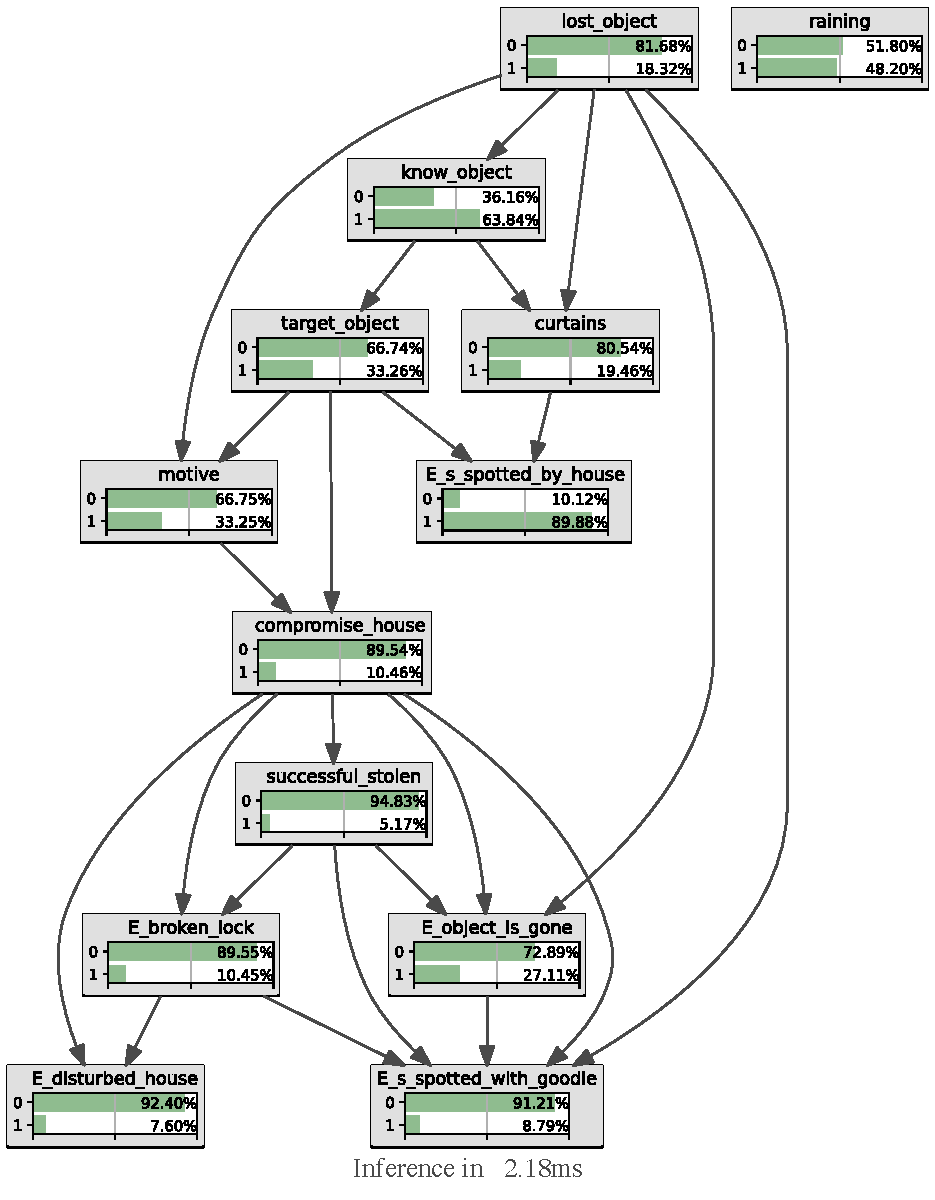
\includegraphics[width=\linewidth]{../experiments/StolenLaptopPrivate/bnImage/BNIMAGEStolenLaptopPrivate.pdf}
\caption{network structure for missing private information}
\label{privatelaptopAcc}
\end{subfigure}
\end{center}

\begin{subfigure}{.45\textwidth}
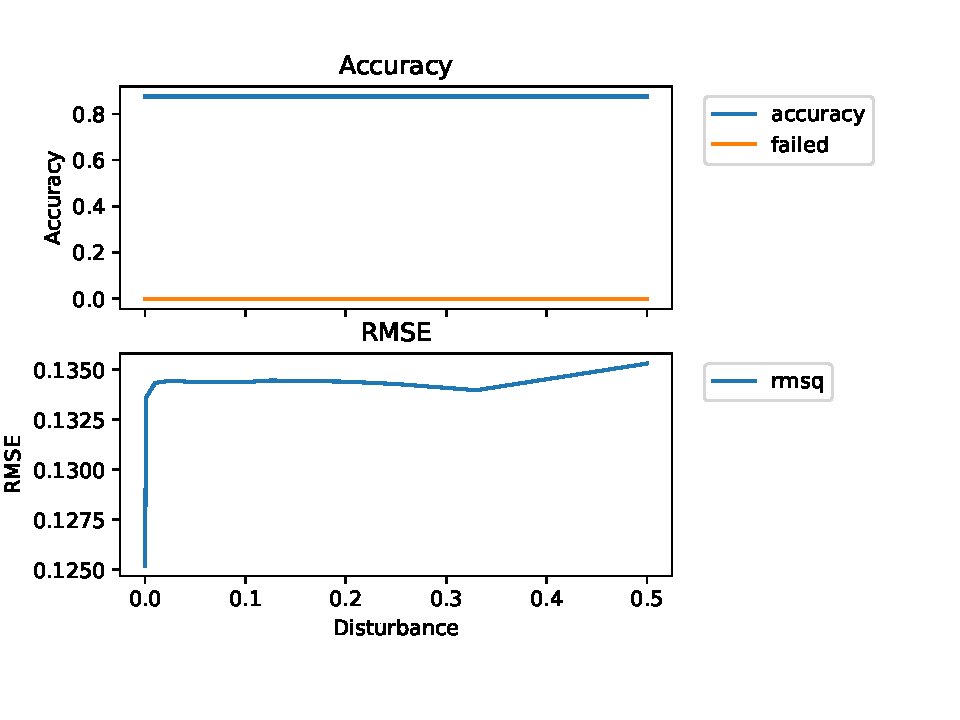
\includegraphics[width=\linewidth]{../experiments/StolenLaptopPrivate/plots/performance_StolenLaptopPrivate.pdf}
\caption{Accuracy (100\% to 0\%) and Root Mean Square error (1 - 0) for missing private information}
\label{privatelaptopAcc}
\end{subfigure}

\begin{subfigure}{.45\textwidth}
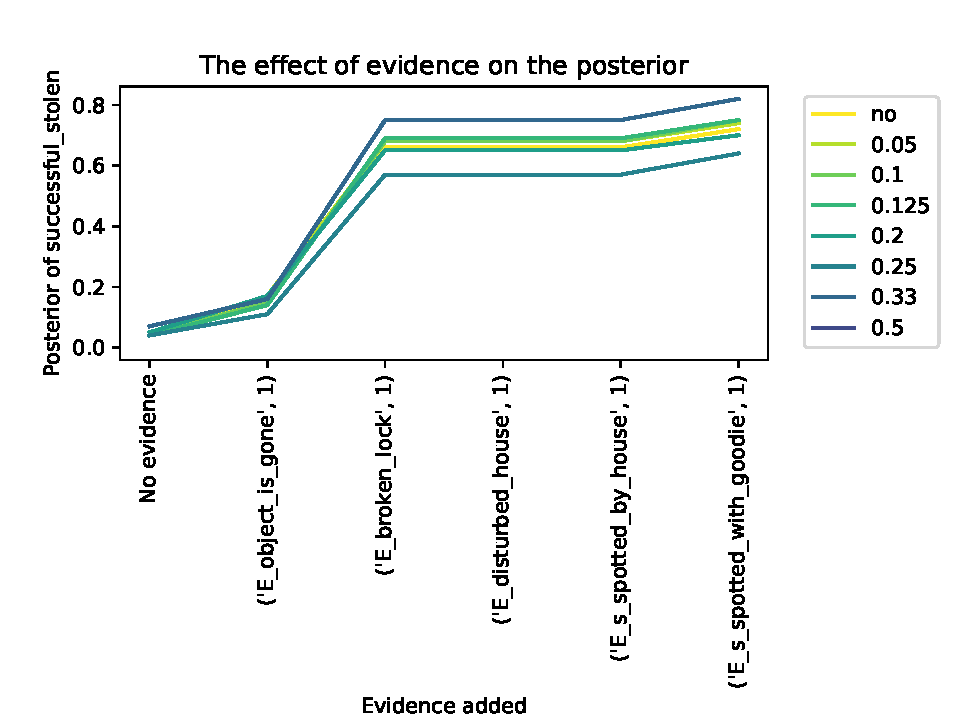
\includegraphics[width=\linewidth]{../experiments/StolenLaptopPrivate/plots/posterior_StolenLaptopPrivate.pdf}
\caption{posterior private information}
\label{privatelaptoppost}
\end{subfigure}

\caption{The network, the accuracy and root mean square for rounding the cpts to intervals, and the effect of evidence on the posterior for stolen laptop simulation.}
\label{private}

\end{figure}


\subsection{Discussion}

Seems to be effective, posterior never goes to 1. Lack of private knowledge hence will affect the end results, even if it will not affect the trajectory of the evidence progression. Overall accuracy and rms performs worse as well.


\section{Conclusion}


{\color{blue} TLDR: We can build an accurate network for a spatial simulation, even when we disturb the cpts. We can see how the posterior probability of an outcome becomes more likely when we add incriminating evidence. We can change parameters in the simulation (change vision radius of camera) and this effects the network (nodes do not show up). We can remove private knowledge, and this reduces the overall accuracy of the network from 100\% to 80\%, although it does not change the `shape' of the effect of the other evidence on the posterior. This all needs to be worked out.}


Simulating works, accuracy and RMS fine.

Table of accuracies and rms for the three experiments for comparisons.

We run into problems when we use words like `near' in our node names. We're lucky that we know what we mean (because our reporter forces us to make this explicit). We do not just ground the probabilities in our network, but we actually also ground our random variables - we have a measure of exactly what events we are interested in, and which we aren't.

We are in trouble with private knowledge, dropping this column from our table (which means that we don't know it) when we make our BN, we're drastically reducing our uh. Accuracy, and increasing our RMS. This implies that we do seem to need a full picture of everything that's happening, otherwise our BN will be kind of terrible, and be less accurate :(.

Hence, for a simulation to work we 1) need to know exactly what it is that we're measuring since evidence strength depends on it \footnote{explain this more}, and 2) private information is necessary to create the BN because it influences fleeing behaviour. If we don't have this information our BN will be less effective.

\subsection{Forensic, Criminal and Legal interpreters, feasibility}
% how will a judge interpret this
If we assume that we can collectively build a network structure like the one that we have now, then there might be a lot of (good) room for legal interpretation. We have shown that this type of Bayesian Network does not have to be very precise. This leaves room for disagreements about probabilities: if we both made a subjective probabilistic estimation, because there's no good data available, and I think something is 20\% likely, and you think it's 30\% likely, we might still be able to agree on 25\%, and this would not result in a large decrease in accuracy of the network. As we've seen, accuracy only starts to decrease at thirds.

In these networks, we see that the evidence updates the posterior in the right direction - more evidence for stealing leads towards a higher value of `successful-stolen'. We also see the effects of different evidence strengths - knowing that the lock is broken is more important than seeing that the house is disturbed.

Forensic scientists will probably be annoyed by the lack of precision, but in these cases we do have a good operationalisation of what exactly is going on. Because we have this operationalisation, we can be sure that our data collection is correct. In the sci-fi world where police builds Bayesian Networks, I can imagine a situation where someone goes over all the files of all the crimes everyday, and collects statistics on occurances. However, the granularity of these crime files and the operationalisation are essential. Here, we can take them for granted. In real life, we cannot and that's a huge problem. 





